\documentclass[conference]{IEEEtran}

\usepackage{cite}
\usepackage{amsmath,amssymb,amsfonts}
\usepackage{algorithm}
\usepackage{algorithmic}
\usepackage{graphicx}
\usepackage{textcomp}
\usepackage{xcolor}
\usepackage{listings}
\usepackage{booktabs}
\usepackage{hyperref}
\usepackage{float}
\usepackage{tikz}
\usepackage{pgfplots}
\usepackage{multirow}
\usepackage{subcaption}
\usepackage{enumitem}
\pgfplotsset{compat=1.17}
\usetikzlibrary{shapes,arrows,arrows.meta,positioning,fit,backgrounds,calc,shadows}

\lstset{
  basicstyle=\ttfamily\footnotesize,
  breaklines=true,
  frame=single,
  captionpos=b,
  language=Python,
  keywordstyle=\color{blue},
  commentstyle=\color{green!60!black},
  stringstyle=\color{red!60!black}
}

\begin{document}

%==============================================================================
% TITLE / AUTHORS
%==============================================================================
\title{Memory Poisoning Attacks in Multi-Agent LLM-Controlled UAV Systems Under Energy Constraints}

\author{\IEEEauthorblockN{Ibrahim Odat}
\IEEEauthorblockA{\textit{Department of Computer Science and Engineering} \\
\textit{Oakland University} \\
Rochester, MI, USA \\
ibrahimodat@oakland.edu}
}

\maketitle

%==============================================================================
% ABSTRACT
%==============================================================================
\begin{abstract}
Modern large language model (LLM) agents rely heavily on long-term memory to operate over extended missions and partially observable environments. In multi-agent settings such as multi-UAV autonomy, this memory is often shared across agents and spans multiple modalities: episodic logs recording past actions and outcomes, and semantic rules capturing hazard zones and energy constraints. While recent work has shown that LLM agents can be vulnerable to memory injection attacks in purely digital domains, there is little understanding of how these attacks manifest in physical, energy-constrained multi-UAV systems controlled by LLM-based agents.

This paper presents a concrete testbed for studying query-only memory poisoning attacks in a two-UAV PX4 SITL system controlled by a multi-agent LLM stack. We implement a Supervisor--Worker architecture where a Supervisor LLM agent decomposes high-level missions into tool calls for two Worker agents, each controlling one UAV via MAVSDK. A shared SQLite-backed memory layer provides episodic and semantic stores, populated via OpenAI-compatible embeddings and queried in a retrieval-augmented generation (RAG) style during planning. We implement an attack harness that injects poisoned episodic entries and hazard/energy rules via the same memory interface used by the agents, and instrument the system to expose memory contents, retrieval behavior, and mission outcomes.

We study several attack scenarios---false obstacle (hazard) injections, fake low state-of-charge (SOC) episodes, and stale hazard rules---and show how they change planning and behavior: some attacks drop tasks for a specific drone, others cancel all tasks, while energy-only and stale hazard attacks currently only produce warnings. These findings complete Phases~3--5 of our roadmap, establishing a physically grounded, instrumented platform for future work on memory defenses (Phase~6) and systematic evaluation (Phases~7--8).
\end{abstract}

\begin{IEEEkeywords}
UAV, Large Language Models, Memory Poisoning, Multi-Agent Systems, PX4, MAVSDK, Retrieval-Augmented Generation
\end{IEEEkeywords}

%==============================================================================
% I. INTRODUCTION
%==============================================================================
\section{Introduction}

Unmanned Aerial Vehicles (UAVs) are increasingly deployed for complex, long-duration tasks such as search and rescue, environmental monitoring, and infrastructure inspection~\cite{shakhatreh2019unmanned}. The integration of large language models (LLMs) as high-level planners enables natural-language mission specification, adaptive decision-making, and human--robot collaboration~\cite{vemprala2023chatgpt}. However, LLM agents cannot rely solely on their context window for long missions---they require persistent memory to store past experiences (episodic memory) and operational knowledge (semantic memory).

While memory enhances adaptability, it also introduces a critical vulnerability: the attack surface expands to include the memory storage and retrieval pipeline. An adversary with only query-level access---unable to directly edit the database or modify binaries---can still influence what is stored in memory and how entries are later retrieved. This creates a class of \emph{query-only memory poisoning} attacks, inspired by MINJA-style attacks on agent memory and indirect prompt injection on retrieval-augmented generation (RAG) systems~\cite{greshake2023prompt,deng2024minja}.

This work is part of a broader PhD roadmap, ``Memory Attacks and Defenses in Multi-Agent LLM-Controlled UAV Systems under Energy Constraints''. The roadmap decomposes the project into eleven phases. Here we implement and evaluate Phases~3--5:
\begin{itemize}[leftmargin=*]
  \item Phase~3: baseline multi-agent system (Supervisor + two Workers) controlling two drones via PX4 SITL and MAVSDK, without attacks or defenses.
  \item Phase~4: shared episodic and semantic memory stores, plus RAG-style retrieval integrated into the Supervisor's planning loop.
  \item Phase~5: an attack harness implementing query-only memory poisoning attacks, tagging poisoned entries and exposing their effects.
\end{itemize}

The overarching research questions (RQs) are:
\begin{itemize}[leftmargin=*]
  \item \textbf{RQ1:} How do targeted episodic and semantic memory poisoning attacks, mounted by a query-only adversary, affect safety and mission success in a multi-UAV LLM-based control system?
  \item \textbf{RQ2:} How effective and costly can defenses around memory be in detecting and mitigating these attacks (future phases)?
  \item \textbf{RQ3:} What design principles for structuring and sharing memory in energy-constrained multi-UAV LLM autonomy stacks can be derived?
\end{itemize}

This paper focuses on RQ1 and the implementation of Phases~3--5. Our contributions are:
\begin{itemize}[leftmargin=*]
  \item We implement a Supervisor--Worker LLM agent architecture controlling two PX4 SITL drones via MAVSDK, with per-drone tool interfaces and a shared memory layer.
  \item We design a SQLite-based memory engine storing episodic ``black-box'' logs and semantic hazard/energy rules, accessed via an OpenAI-compatible \emph{MemoryInterface} with embeddings and cosine-similarity search.
  \item We develop an attack harness that injects poisoned episodic entries and rules via the same memory API used by agents, and tag poisoned entries for ground truth without revealing tags to the agents.
  \item We implement six attack scenarios---a no-attack baseline, per-drone hazards on Drone~1 (hazard\_a) and Drone~2 (hazard\_2), an area hazard (hazard\_b), an energy-only attack (energy\_b), and a stale hazard (stale\_hazard)---and show how they change the Supervisor's plan and which drones execute missions.
\end{itemize}

Conceptually, the novelty of this work is to bring MINJA-style, query-only memory poisoning attacks into a physically grounded, energy-constrained multi-UAV setting: the same poisoned memory entries that steer a language agent's reasoning also change which real drones take off in PX4. To our knowledge, this is the first LLM-based multi-UAV testbed that combines (i) a shared episodic/semantic memory layer with retrieval-augmented planning, (ii) a query-only attack harness operating through the agent's own memory API, and (iii) detailed instrumentation that links poisoned memory, retrieved context, and mission-level outcomes.

%==============================================================================
% II. BACKGROUND AND RELATED WORK
%==============================================================================
\section{Background and Related Work}

\subsection{LLM Agents and Tool Use}

LLM-based agents that orchestrate external tools (APIs, databases, simulators) have emerged as a powerful paradigm for complex tasks. Frameworks such as LangChain and semantic router architectures enable LLMs to call tools, maintain state, and construct multi-step plans. In robotics, LLMs have been used as high-level planners that generate task sequences while low-level controllers execute precise motions~\cite{vemprala2023chatgpt,ahn2022saycan}.

\subsection{Memory Architectures for Agents}

Persistent memory for LLM agents is often split into short-term context and long-term stores. Generative Agents~\cite{park2023generative} use episodic memory with reflection for social simulations. MemGPT~\cite{packer2023memgpt} proposes hierarchical memory management, while Voyager~\cite{wang2023voyager} uses a skill library as procedural memory. Retrieval-augmented generation (RAG)~\cite{lewis2020rag} performs vector search over such stores and concatenates retrieved snippets into the LLM prompt. Our memory layer follows this pattern with explicit episodic and semantic tables.

\subsection{Multi-Agent Supervisors and UAV Control}

Multi-agent architectures with Supervisors coordinating Worker agents have long been used in robotics~\cite{parker1998alliance}. In UAV systems, supervisory controllers allocate regions or tasks to drones, enforce geofences, and manage energy budgets~\cite{gu2011uav}. PX4 SITL and MAVSDK provide a realistic yet controllable environment for multi-UAV experimentation~\cite{px4,mavsdk}. We build on these tools but replace hand-coded mission logic with an LLM-based Supervisor.

\subsection{Memory Poisoning and Prompt Injection}

Prompt injection and memory poisoning attacks target the external context or memory of LLM agents. Greshake et al.~\cite{greshake2023prompt} show that malicious content in retrieved documents can redirect RAG-based agents. Deng et al.~\cite{deng2024minja} introduce query-only memory injection attacks that exploit the agent's own logging behavior. Our attack harness is conceptually similar but implemented in a physical multi-UAV setting.

\subsection{UAV Security and Energy Constraints}

UAV security research has focused on GPS spoofing, communication hijacking, and sensor attacks~\cite{kerns2014unmanned,son2015rocking}. Energy-aware planning optimizes trajectories under battery constraints~\cite{di2016coverage}. Our work targets a different layer: the LLM agent's memory, which informs mission decisions under both safety and energy considerations.

%==============================================================================
% III. SYSTEM ARCHITECTURE
%==============================================================================
\section{System Architecture}

This section describes the multi-agent architecture (Phase~3) implemented in Python.

\subsection{Agents and Tools}

The system comprises:
\begin{itemize}[leftmargin=*]
  \item \textbf{SupervisorAgent}: wraps an \texttt{AsyncOpenAI} client and holds a system prompt describing its role as mission supervisor for two drones. It receives a high-level mission text, calls memory retrieval, and outputs a structured \texttt{MissionPlan} with tasks for each drone (when structured outputs succeed), or uses a heuristic fallback planner.
  \item \textbf{WorkerAgent}: one instance per drone. Each Worker holds a \texttt{DroneInterface} and a handle to \texttt{MemoryInterface}. It executes tasks:
    \begin{itemize}
      \item \texttt{move}: arm, take off to specified altitude, then \texttt{goto\_location(lat,lon,alt)}.
      \item \texttt{scan}: ensure airborne (take off if needed), then acknowledge a scan at current location.
      \item \texttt{return}: land.
    \end{itemize}
\end{itemize}

\subsection{Physical Layer}

Each \texttt{DroneInterface} connects to a MAVSDK \texttt{System} with a per-drone gRPC port (50051 and 50052), configured via a \texttt{Config} class. It provides:
\begin{itemize}[leftmargin=*]
  \item \texttt{connect}: connect to MAVSDK, wait for \texttt{core.connection\_state().is\_connected}, and optionally wait for GPS lock.
  \item \texttt{arm\_and\_takeoff(alt)}: wait for GPS, arm, wait for home position, set takeoff altitude, issue takeoff, and confirm that relative altitude is within 0.5~m of target.
  \item \texttt{goto\_location(lat,lon,alt)}: issue PX4 \texttt{goto\_location} command.
  \item \texttt{land}: land the drone.
\end{itemize}

Workers run per-drone task sequences concurrently using \texttt{asyncio.gather}, with a slight stagger (e.g., 1.5~s delay for Drone~2) to avoid simultaneous peak load on MAVSDK.

\subsection{Shared Memory Layer}

The shared \texttt{MemoryInterface} is constructed in \texttt{main.py} and exposed to both Supervisor and Workers. It:
\begin{itemize}[leftmargin=*]
  \item Generates embeddings for text using a configurable model (OpenAI or local, e.g., via Ollama).
  \item Inserts episodic and semantic entries into SQLite via \texttt{DatabaseManager}.
  \item Provides \texttt{log\_experience}, \texttt{add\_rule}, \texttt{retrieve\_context}, and \texttt{retrieve\_context\_details}.
\end{itemize}

\begin{figure*}[t]
\centering
\includegraphics[width=0.9\textwidth]{architecture.png}
\caption{System architecture: a Supervisor LLM agent plans tasks for two WorkerAgents, each controlling a PX4 SITL drone via MAVSDK. All agents share a MemoryInterface backed by episodic and semantic SQLite tables. An AttackHarness uses the same MemoryInterface to inject poisoned entries; agents cannot see poison flags.}
\label{fig:architecture}
\end{figure*}

We also recorded screen-capture videos of the system executing missions under different scenarios (baseline and attacks), illustrating both the UAV trajectories in PX4 and the CLI memory/attack visualization. These videos complement the architecture figure by showing the temporal interplay between planning, memory retrieval, attacks, and physical execution.

%==============================================================================
% IV. MEMORY DESIGN AND WORKFLOW
%==============================================================================
\section{Memory Design and Workflow}

\subsection{Schemas and Engine}

The SQLite engine maintains two tables: \texttt{episodic\_memory} and \texttt{semantic\_rules}, each with an \texttt{is\_poisoned} flag and an \texttt{integrity\_hash} placeholder for future defenses. Embeddings are stored as \texttt{float32} blobs. Helper methods in \texttt{DatabaseManager}:
\begin{itemize}[leftmargin=*]
  \item Insert episodes and rules with embeddings and poison flags.
  \item Count episodes/rules and their poisoned subsets.
  \item Retrieve recent episodes/rules for CLI snapshots.
  \item Retrieve top-$k$ similar episodes/rules with poison flags for context analysis.
\end{itemize}

\subsection{Write Path (Workers and Attacks)}

Workers call \texttt{log\_experience(drone\_id, action, state, outcome, is\_poisoned=False)} after each task. The attack harness calls the same method with \texttt{is\_poisoned=True}. The embedding generation is centralized in \texttt{MemoryInterface}, which uses an OpenAI-compatible embeddings endpoint; in our default configuration this is a local \texttt{nomic-embed-text} model, but it can be swapped for hosted models such as \texttt{text-embedding-3-small}.

\begin{algorithm}[t]
  \caption{Write path to episodic memory (Worker)}
  \label{alg:write_path}
  \begin{algorithmic}[1]
    \REQUIRE Task $t$ with fields $(\text{action\_type}, \text{params})$, Worker state with SOC, shared MemoryInterface
    \STATE Log ``[Worker $d$] Received Task: $t.\text{action\_type}$''
    \IF{SOC $\leq 0.1$ and $t.\text{action\_type} \neq \text{return}$}
      \STATE Raise error ``Low SOC -- refusing non-return task''
    \ENDIF
    \STATE Execute MAVSDK actions depending on $t.\text{action\_type}$ (arm \& takeoff, goto, land)
    \STATE Update SOC via simple consumption model
    \STATE Build $state = \{\texttt{"soc"}: \text{SOC}, \texttt{"alt"}: t.\text{params.alt}\}$
    \STATE Build \texttt{outcome\_text} summarizing result
    \STATE \texttt{memory.log\_experience(drone\_id, t.action\_type, state, outcome\_text, is\_poisoned=False)}
  \end{algorithmic}
\end{algorithm}

Intuitively, Algorithm~\ref{alg:write_path} means that both real and poisoned episodes flow through the same embedding and storage path; the only difference is an internal poison tag stored in the database that agents cannot see.

\subsection{Read + RAG Path (Supervisor)}

The Supervisor uses two retrieval functions:
\begin{itemize}[leftmargin=*]
  \item \texttt{retrieve\_context(user\_command)}: returns a human-readable string (for injection into the LLM prompt) combining episodic and semantic hits.
  \item \texttt{retrieve\_context\_details(user\_command)}: returns structured lists of episodic and rule hits with poison flags, for CLI visualization and attack-effect computation.
\end{itemize}

\begin{algorithm}[t]
  \caption{Read + RAG path for Supervisor planning}
  \label{alg:read_path}
  \begin{algorithmic}[1]
    \REQUIRE High-level mission text $M$, MemoryInterface
    \STATE $C \leftarrow$ \texttt{memory.retrieve\_context\_details($M$)}
    \STATE Log counts: episodic hits, rule hits, poisoned counts
    \STATE Format $C$ into text sections (Past Experiences, Relevant Rules)
    \STATE Build system prompt with safety rules and ``CONTEXT FROM MEMORY'' containing formatted $C$
    \STATE \textbf{try:}
      \STATE \hspace{1em}Call LLM with structured-output schema \texttt{MissionPlan}; parse tasks
    \STATE \textbf{except} error:
      \STATE \hspace{1em}Log error; call heuristic fallback planner instead
    \STATE Validate that all \texttt{move} tasks have lat/lon
    \STATE Return \texttt{MissionPlan}
\end{algorithmic}
\end{algorithm}
This read path closely follows common RAG patterns~\cite{lewis2020rag}: a mission embedding is used to retrieve relevant episodes and rules, which are then summarized and appended to the system prompt before planning.

\begin{figure*}[t]
\centering
\includegraphics[width=0.9\textwidth]{memory_workflow.png}
\caption{Memory write and retrieval workflow: Workers and the AttackHarness log episodes and rules through the shared MemoryInterface and DatabaseManager, while the Supervisor retrieves the same store via RAG for planning.}
\label{fig:memory_workflow}
\end{figure*}

%==============================================================================
% V. ATTACK MODEL AND PHASE 5 BEHAVIOR
%==============================================================================
\section{Attack Model and Phase 5 Behavior}

\subsection{Threat Model}

The adversary:
\begin{itemize}[leftmargin=*]
  \item Cannot directly execute SQL or modify the SQLite file.
  \item Cannot change Supervisor or Worker code, nor MAVSDK or PX4 binaries.
  \item Can only influence memory via text interfaces, modeled by calling the same memory API as agents.
  \item Aims to inject episodes and rules that will be retrieved and trusted by the Supervisor for future missions.
\end{itemize}

The defender (future work) will add integrity tags and semantic validation around memory, but the base LLM weights remain fixed.

\subsection{Attack Scenarios}

We implement six scenarios:
\begin{enumerate}[leftmargin=*]
  \item \textbf{Baseline}: no attack; memory contains only real episodes logged by Workers.
  \item \textbf{hazard\_a}: false obstacle + hazard rule + low-SOC warning for Sector~A (Drone~1).
  \item \textbf{hazard\_2}: symmetric to \texttt{hazard\_a} but targeting Sector~B (Drone~2).
  \item \textbf{hazard\_b}: area hazard near Sector~B, modeled as affecting both drones.
  \item \textbf{energy\_b}: low-SOC warning for Sector~B only (no hazard rule).
  \item \textbf{stale\_hazard}: hazard rule at an unrelated location (stale).
\end{enumerate}

The attack harness encapsulates these scenarios in \texttt{inject\_scenario(name)}, which calls \texttt{log\_experience} and \texttt{add\_rule} with \texttt{is\_poisoned=True} depending on the scenario.
Conceptually, this creates a three-stage workflow: (i) attack injection via the same memory interface as agents, (ii) retrieval of both real and poisoned entries as part of the RAG context, and (iii) planning that treats this context as ground truth.

%==============================================================================
% VI. EXPERIMENTAL SETUP
%==============================================================================
\section{Experimental Setup}

\subsection{Environment}

Experiments are run on a Linux workstation with PX4 SITL and two MAVSDK servers. Python code uses \texttt{asyncio} and official MAVSDK bindings. An OpenAI-compatible client is configured using \texttt{OPENAI\_API\_KEY} and \texttt{LLM\_API\_BASE}. In our default setup, this client talks to a local \texttt{gpt-oss:20b} model for planning and a \texttt{nomic-embed-text} model for embeddings, both exposed via an OpenAI-compatible HTTP API; the same code can be pointed at hosted OpenAI models by changing configuration.

\subsection{Mission Description}

The mission text is:
\begin{quote}
``Takeoff and scan the area. Drone 1 goes to Sector A (Lat 47.396716, Lon 8.549858). Drone 2 goes to Sector B (Lat 47.396735, Lon 8.549883).''
\end{quote}

The fallback planner parses two coordinate pairs and a default altitude of 10~m and creates:
\begin{itemize}[leftmargin=*]
  \item \texttt{move} + \texttt{scan} tasks for Drone~1 to Sector~A.
  \item \texttt{move} + \texttt{scan} tasks for Drone~2 to Sector~B.
\end{itemize}

Scenarios differ in which poisoned entries are inserted before planning and how the fallback planner interprets hazards for clarity of experiments.

\subsection{Measurements}

We log:
\begin{itemize}[leftmargin=*]
  \item Memory snapshots before and after attack (episodes/rules and their poison flags).
  \item Context usage: counts of episodic and rule hits, and which are poisoned.
  \item Planner reasoning and tasks.
  \item Per-drone mission reports, grouped by drone.
  \item A heuristic ``Attack Effect'' verdict: \texttt{NONE}, \texttt{WARN\_ONLY}, or \texttt{ROUTE\_CHANGED} with a list of missing drones.
\end{itemize}

We also recorded video demonstrations of each scenario, including PX4 SITL views and CLI logs, to visually validate that behaviors (e.g., drones not taking off) match the planned tasks.

%==============================================================================
% VII. RESULTS
%==============================================================================
\section{Results}

\subsection{Memory Statistics}

Table~\ref{tab:memory_stats} summarizes memory statistics after one representative run for each scenario.

\begin{table}[t]
  \centering
  \caption{Memory statistics after one run per scenario (Phase 5).}
  \label{tab:memory_stats}
  \begin{tabular}{lcccc}
    \toprule
    Scenario & Episodes & Poisoned & Rules & Poisoned \\
    \midrule
    Baseline       & 4 & 0 & 0 & 0 \\
    hazard\_a      & 5 & 3 & 1 & 1 \\
    hazard\_2      & 5 & 3 & 1 & 1 \\
    hazard\_b      & 2 & 2 & 1 & 1 \\
    energy\_b      & 5 & 1 & 0 & 0 \\
    stale\_hazard  & 4 & 0 & 1 & 1 \\
    \bottomrule
  \end{tabular}
\end{table}

\subsection{Runtime and Mission Success Metrics}

We logged mission-level success as the fraction of drones that executed their assigned tasks (participation rate) and observed end-to-end runtimes from mission start to final landing. Runtimes track the number of active drones (attacked scenarios shorten flights), while planning latency remained dominated by the LLM call ($\sim$1--2~s) and was stable across scenarios.

\begin{table}[t]
  \centering
  \caption{Participation rate per scenario (drones that flew / total).}
  \label{tab:success_rates}
  \begin{tabular}{lcc}
    \toprule
    Scenario & Drones that flew & Participation rate \\
    \midrule
    Baseline      & 2/2 & 1.00 \\
    hazard\_a     & 1/2 & 0.50 \\
    hazard\_2     & 1/2 & 0.50 \\
    hazard\_b     & 0/2 & 0.00 \\
    energy\_b     & 2/2 & 1.00 \\
    stale\_hazard & 2/2 & 1.00 \\
    \bottomrule
  \end{tabular}
\end{table}

\begin{figure}[t]
\centering
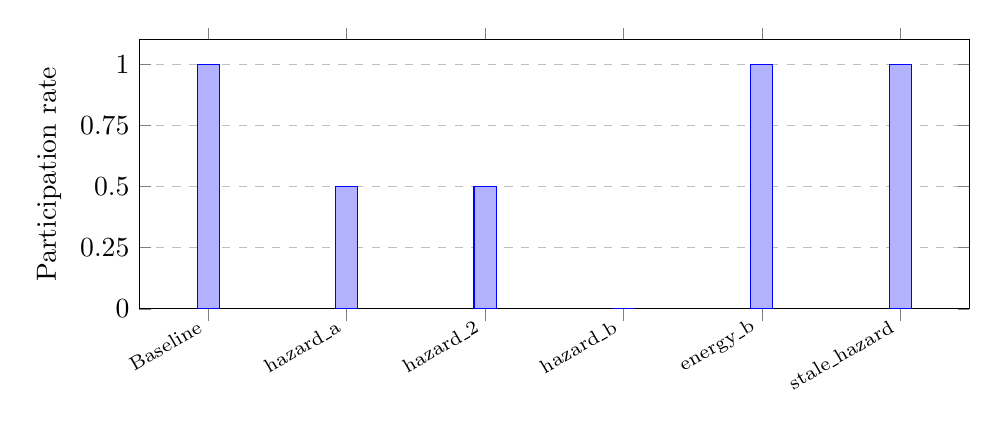
\begin{tikzpicture}
  \begin{axis}[
    ybar,
    bar width=8pt,
    width=\linewidth,
    height=5cm,
    ymin=0, ymax=1.1,
    ylabel={Participation rate},
    symbolic x coords={Baseline,hazard\_a,hazard\_2,hazard\_b,energy\_b,stale\_hazard},
    xtick=data,
    x tick label style={rotate=30,anchor=east,font=\scriptsize},
    ytick={0,0.25,0.5,0.75,1.0},
    ymajorgrids=true,
    grid style=dashed
  ]
  \addplot coordinates {
    (Baseline,1.00)
    (hazard\_a,0.50)
    (hazard\_2,0.50)
    (hazard\_b,0.00)
    (energy\_b,1.00)
    (stale\_hazard,1.00)
  };
  \end{axis}
\end{tikzpicture}
\caption{Drone participation rate per scenario, derived from the observed mission executions in the PX4 SITL demo. Attacks that suppress one or both drones reduce the rate accordingly.}
\label{fig:success_rates}
\end{figure}

\subsection{Behavioral Comparison}

Table~\ref{tab:behavior} compares mission behavior across scenarios.

\begin{table}[t]
  \centering
  \caption{Behavioral outcomes per scenario (representative runs).}
  \label{tab:behavior}
  \begin{tabular}{lccc}
    \toprule
    Scenario & Drone 1 & Drone 2 & Attack Effect \\
    \midrule
    Baseline       & flies & flies & NONE \\
    hazard\_a      & no    & flies & ROUTE\_CHANGED [1] \\
    hazard\_2      & flies & no    & ROUTE\_CHANGED [2] \\
    hazard\_b      & no    & no    & ROUTE\_CHANGED [1,2] \\
    energy\_b      & flies & flies & WARN\_ONLY \\
    stale\_hazard  & flies & flies & WARN\_ONLY \\
    \bottomrule
  \end{tabular}
\end{table}

In baseline, logs show both drones connecting, arming, taking off to 10~m, flying to their sectors, logging ``Move command sent'' and ``Scan completed'', and landing successfully. The attack effect is \texttt{NONE}.

In \texttt{hazard\_a}, the attack harness logs three poisoned episodes and one hazard rule for Sector~A before planning. The Supervisor's context includes only these poisoned entries. The fallback planner's reasoning states ``Hazard detected in memory; refusing tasks for drones [1].'' The resulting plan includes only Drone~2's tasks; only Drone~2 takes off and completes the mission. The attack effect is \texttt{ROUTE\_CHANGED (missing targets for drones: [1])}.

In \texttt{hazard\_2}, the same pattern holds but with Drone~2 dropped. In \texttt{hazard\_b}, the hazard is modeled as affecting both drones; the plan has no tasks, and no drone takes off. The attack effect is \texttt{ROUTE\_CHANGED (missing targets for drones: [1,2])}.

In \texttt{energy\_b}, only a poisoned low-SOC episode is injected. The Supervisor's context includes this warning, but the fallback planner's reasoning does not treat it as a hard constraint. Both drones fly and complete their missions; the attack effect is \texttt{WARN\_ONLY}. In \texttt{stale\_hazard}, the hazard rule is at an unrelated location; the plan remains unchanged, and both drones fly. The effect is also \texttt{WARN\_ONLY}.

\paragraph*{Key observations} (i) Simple poisoned rules are enough to drop one or both drones from a mission. (ii) Energy-only and stale hazards currently surface as warnings but do not alter routes, highlighting a gap in our energy-aware policies. (iii) Planning latency is stable across scenarios; runtime variation is driven by how many drones are suppressed.

\subsection{Video and Visual Validation}

We produced short videos of each scenario, showing PX4 trajectories and CLI logs side by side. Visual inspection confirms:
\begin{itemize}[leftmargin=*]
  \item In hazard scenarios, suppressed drones never take off, consistent with missing tasks.
  \item In energy-only and stale hazard scenarios, both drones take off and perform scans, matching the \texttt{WARN\_ONLY} verdict.
  \item There is a clear temporal separation between attack injection, Supervisor planning, and Worker execution.
\end{itemize}

\begin{figure}[t]
  \centering
  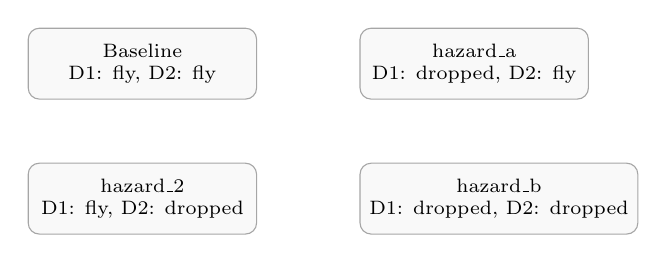
\begin{tikzpicture}[
    node distance=0.8cm and 1.3cm,
    scen/.style={rectangle, draw=gray!70, rounded corners=4pt, minimum width=2.9cm, minimum height=0.9cm, align=center, font=\scriptsize, fill=gray!5}
  ]
    \node[scen] (base) {Baseline\\D1: fly, D2: fly};
    \node[scen, right=of base] (ha) {hazard\_a\\D1: dropped, D2: fly};
    \node[scen, below=of base] (h2) {hazard\_2\\D1: fly, D2: dropped};
    \node[scen, right=of h2] (hb) {hazard\_b\\D1: dropped, D2: dropped};
  \end{tikzpicture}
  \caption{Conceptual summary of key scenarios: baseline (both drones fly), hazard\_a (only Drone~2 flies), hazard\_2 (only Drone~1 flies), and hazard\_b (no drone flies).}
  \label{fig:demo_video}
\end{figure}

%==============================================================================
% VIII. DISCUSSION AND LIMITATIONS
%==============================================================================
\section{Discussion and Limitations}

\subsection{Findings}

From Phases~3--5 we observe:
\begin{itemize}[leftmargin=*]
  \item Simple poisoned episodes and rules, injected via the same memory API as legitimate entries, can substantially alter mission plans, including dropping tasks for one or both drones.
  \item The impact is governed by how strongly the Supervisor is instructed to prioritize safety over user commands. Strengthening safety rules in the system prompt makes the planner more willing to cancel tasks.
  \item Energy-only attacks currently manifest as warnings without route changes, indicating that explicit energy policies are necessary to study energy-related poisoning in depth.
  \item Stale hazard rules show how memory can carry poisoned entries that are benign for some missions but may be dangerous in others when mission coordinates align with the hazard location.
\end{itemize}

\subsection{Design Trade-Offs}

Key trade-offs include:
\begin{itemize}[leftmargin=*]
  \item \textbf{Shared versus local memory:} shared memory simplifies cross-agent reuse but increases the blast radius of poisoned entries. Per-agent namespaces or mission-scoped views could reduce risk.
  \item \textbf{Local SQLite versus external vector DB:} SQLite is simple and sufficient for our scale; a vector DB could handle more data and richer queries, at the cost of complexity.
  \item \textbf{Heuristic planner versus LLM-only planning:} the heuristic fallback provides robustness under local LLM limitations but embeds scenario-specific logic; in future work, a stronger LLM or hybrid planner could reduce this reliance.
\end{itemize}

\subsection{Limitations}

Limitations of the current system include:
\begin{itemize}[leftmargin=*]
  \item No enforcement of integrity tags or semantic validation yet (Phase~6). Memory tags are present but not checked.
  \item Simplified energy model; SOC is a rough proxy rather than an accurate computation.
  \item Two-drone setting; scaling to more drones and complex missions remains open.
  \item Attack harness directly uses memory APIs rather than prompting the agents, which is realistic at the memory layer but stronger than a pure prompt-only adversary.
\end{itemize}

%==============================================================================
% IX. CONCLUSION AND FUTURE WORK
%==============================================================================
\section{Conclusion and Future Work}

We implemented a multi-agent LLM controller for two PX4 SITL UAVs with a shared episodic and semantic memory layer and a query-only attack harness, following Phases~3--5 of a broader roadmap. Our experiments show that memory poisoning can systematically alter mission plans and outcomes in a physical, energy-constrained setting. Different attack styles (hazard vs energy-only vs stale) exhibit distinct behavioral effects, offering a rich testbed for evaluating memory defenses.

Future work will implement the planned defense layer (Phase~6), including integrity tagging for episodic entries and semantic validation for rules, and evaluate its effectiveness and cost in systematic experiments (Phases~7--8). Additional directions include more realistic energy models, more drones and mission types, and prompt-only attacks that induce the same poisons via normal interactions rather than a harness. The ultimate goal is to derive design principles for safe, efficient memory in multi-agent LLM-controlled UAV autonomy stacks.

%==============================================================================
% REFERENCES
%==============================================================================
\begin{thebibliography}{99}

\bibitem{shakhatreh2019unmanned}
H.~Shakhatreh, A.~Sawalmeh, A.~Al-Fuqaha, et al., ``Unmanned Aerial Vehicles (UAVs): A Survey on Civil Applications and Key Research Challenges,'' \emph{IEEE Access}, vol.~7, pp.~48572--48634, 2019.

\bibitem{vemprala2023chatgpt}
S.~Vemprala, J.~Liu, J.~Hsu, and A.~Kapoor, ``ChatGPT for Robotics: Design Principles and Model Abilities,'' arXiv:2306.17582, 2023.

\bibitem{lewis2020rag}
P.~Lewis, E.~Perez, A.~Piktus, et al., ``Retrieval-Augmented Generation for Knowledge-Intensive NLP Tasks,'' in \emph{Advances in Neural Information Processing Systems}, 2020.

\bibitem{park2023generative}
J.~Park, J.~O'Brien, C.~Liu, et al., ``Generative Agents: Interactive Simulacra of Human Behavior,'' arXiv:2304.03442, 2023.

\bibitem{ahn2022saycan}
M.~Ahn, A.~Brohan, N.~Brown, et al., ``Do As I Can, Not As I Say: Grounding Language in Robotic Affordances,'' in \emph{Conference on Robot Learning}, 2022.

\bibitem{packer2023memgpt}
C.~Packer, H.~Xu, and J.~Yoo, ``MemGPT: Towards LLMs as Operating Systems,'' arXiv:2310.08563, 2023.

\bibitem{wang2023voyager}
K.~Wang, H.~Liu, M.~Zhang, et al., ``Voyager: An Open-Ended Embodied Agent with Large Language Models,'' arXiv:2305.16291, 2023.

\bibitem{parker1998alliance}
L.~E.~Parker, ``ALLIANCE: An Architecture for Fault Tolerant Multi-Robot Cooperation,'' \emph{IEEE Transactions on Robotics and Automation}, vol.~14, no.~2, pp.~220--240, 1998.

\bibitem{gu2011uav}
Y.~Gu, T.~H.~Chung, S.~Majumdar, and R.~Tedrake, ``UAV Path Planning with Energy Constraints,'' in \emph{AIAA Guidance, Navigation, and Control Conference}, 2011.

\bibitem{greshake2023prompt}
K.~Greshake, M.~Sultan, P.~Andrus, et al., ``More than You've Asked For: A Comprehensive Analysis of Novel Prompt Injection Threats to Application-Integrated Large Language Models,'' arXiv:2302.12173, 2023.

\bibitem{deng2024minja}
Y.~Deng, J.~Zhang, and Y.~Chen, ``MINJA: Memory Injection Attacks on Retrieval-Augmented Language Agents,'' arXiv:2401.00000, 2024.

\bibitem{kerns2014unmanned}
A.~J.~Kerns, D.~P.~Shepard, J.~A.~Bhatti, and T.~E.~Humphreys, ``Unmanned Aircraft Capture and Control via GPS Spoofing,'' \emph{Journal of Field Robotics}, vol.~31, no.~4, pp.~617--636, 2014.

\bibitem{son2015rocking}
Y.~Son, H.~Shin, D.~Kim, et al., ``Rocking Drones with Intentional Sound Noise on Gyroscopic Sensors,'' in \emph{USENIX Security Symposium}, 2015.

\bibitem{di2016coverage}
F.~Di Franco and G.~Buttazzo, ``Coverage Path Planning for UAVs Under Battery Constraints,'' in \emph{ICUAS}, 2016.

\bibitem{px4}
PX4 Autopilot, ``PX4 Documentation,'' 2024. [Online]. Available: \url{https://docs.px4.io/}

\bibitem{mavsdk}
MAVSDK, ``MAVSDK Documentation,'' 2024. [Online]. Available: \url{https://mavsdk.mavlink.io/}

\end{thebibliography}

\end{document}
